\section{Theorie}
\label{sec:Theorie}
\subsection{Problemstellung}
\label{sec:problemstellung}
Eine Kraft, die an eine Oberfläche angreift, erzeugt pro Flächeneinheit eine Spannung.
Diese kann senkrecht oder aber tangential zu der Oberfläche wirken und wird dann
Normalspannung oder Tangential- beziehungsweise Schubspannung genannt.
Der Zusammenhang zwischen der Normalspannung $\sigma$ und
der erzeugten Längenänderung $\Delta L/L$ eines Körpers wird beschrieben durch das Hookesche Gesetz.
Es ergibt sich zu
\begin{equation}
  \sigma = E \frac{\Delta L}{L}.
  \label{eqn:captainhook}
\end{equation}
Hierbei meint $E$ das Elastizitätsmodul, einen Proportionalitätsfaktor, der eine
Materialkonstante des jeweiligen Körpers ist und der experimentell mithilfe der
Biegung eines Körpers bestimmt werden kann.
Hierfür beschreibt man die Biegung mit einer Funktion $D(x)$. Für diese gilt
\begin{equation}
  D(x) = D_G(x) + D_0(x).
  \label{eqn:DmitNull}
\end{equation}
Hierbei bezeichnet $D_G(x)$ die Auslenkung bei einem angehängten Gewicht an den Körper
und $D_0(x)$ die Auslenkung des Körpers in der Ruhelage ohne ein angehängtes Gewicht.
Um die Funktion zu bestimmen, können zwei Verfahren verwendet werden. Auf diese
wird im Folgenden näher eingegangen.

\subsection{Berechnung der Durchbiegung bei einseitiger Aufhängung}
\label{sec:einseitigg}
Im folgenden Abschnitt wird die Durchbiegung eines homogenen Stabes bei einseitiger
Einspannung nach in Abbildung \ref{fig:einseitig} dargestelltem Aufbau untersucht,
um die Funktion $D(x)$ sowie das Elastizitätsmodul zu erhalten.
\begin{figure}[H]
  \centering
  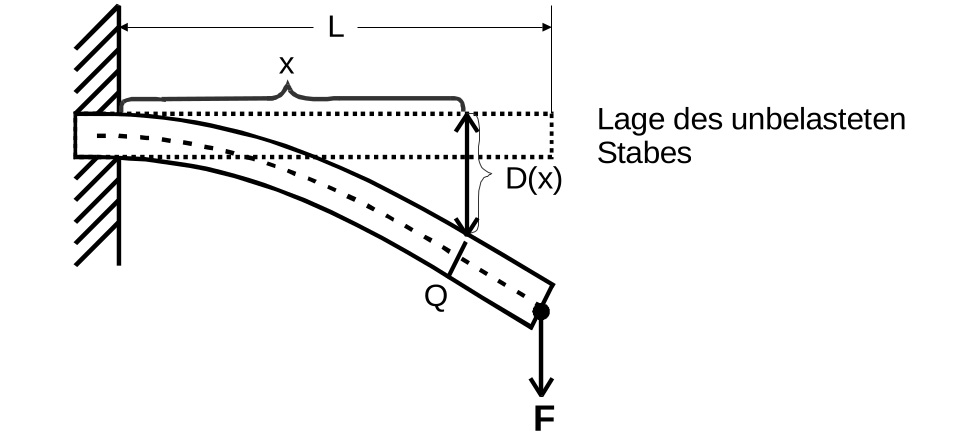
\includegraphics[scale=0.4]{content/EinspannungEinseitig.png}
  \caption{Durchbiegung eines elastischen Stabes bei einseitiger Einspannung. \cite{AP01}}
  \label{fig:einseitig}
\end{figure}
\noindent
Durch ein angehängtes Gewicht wird ein Drehmoment $M_F$ auf den Querschnitt $Q$ des
Stabes ausgeübt. Aufgrund der Elastizität des Stabes wirken diesem Drehmoment im
inneren des Stabes Normalspannungen entgegen. Diese erzeugen ein Drehmoment $M_\sigma$.
Innerhalb des Stabes gibt es eine neutrale Faser, in der keinerlei Spannungen auftreten.
Unter Vernachlässigung des durch das Eigengewicht des Stabes erzeugten Drehmoments
ergibt sich eine Gleichgewichtslage, in der gilt
\begin{equation}
  M_F = M_\sigma .
  \label{eqn:momentengleichung1}
\end{equation}
Hierbei lässt sich $M_\sigma$ durch Integration über den Querschnitt $Q$ des Stabes
ermitteln:
\begin{equation}
  M_\sigma = \int_Q  y \sigma(y) dq.
  \label{eqn:msigma}
\end{equation}
$y$ meint hier den Abstand des Flächenelementes $dq$ von der neutralen Faser
des Stabes $x$ sowie $\sigma(y)$ die Normalspannung.
$M_F$ wirkt durch die Länge $L$ des Stabes mit einem Hebel, weshalb sich der Betrag des Drehmoments
$M_F$ wie folgt bestimmen lässt:
\begin{equation}
  M_F = F(L - x).
  \label{eqn:mf}
\end{equation}
Daher ergibt sich die auch als Momentengleichung bezeichnete Gleichung \eqref{eqn:momentengleichung1}
mit Gleichung \eqref{eqn:msigma} sowie Gleichung \eqref{eqn:mf} zu
\begin{equation}
  F(L - x) = \int_Q  y \sigma(y) dq.
  \label{eqn:momentengleichung2}
\end{equation}
Die hier auftretende Normalspannung $\sigma(y)$ lässt sich nach dem Hookeschen Gesetz \eqref{eqn:captainhook} bestimmen.
Sie ergibt sich zu
\begin{equation}
  \sigma(y) = E \frac{\delta x}{\Delta x}.
  \label{eqn:normalspannung}
\end{equation}
$y$ gibt hier den Abstand zu der neutralen Faser des Stabes der Länge $\Delta x$ an.
Durch die Durchbiegung entsteht eine Längenänderung der neutralen Faser von $\Delta x$ zu $\delta x$.
Diese Längenänderung ergibt sich nach Abbildung \ref{fig:einspannungeinseitig2} zu
\begin{equation}
  \delta x = y \frac{\Delta x}{R}.
  \label{eqn:kleindeltax}
\end{equation}
\begin{figure}[H]
  \centering
  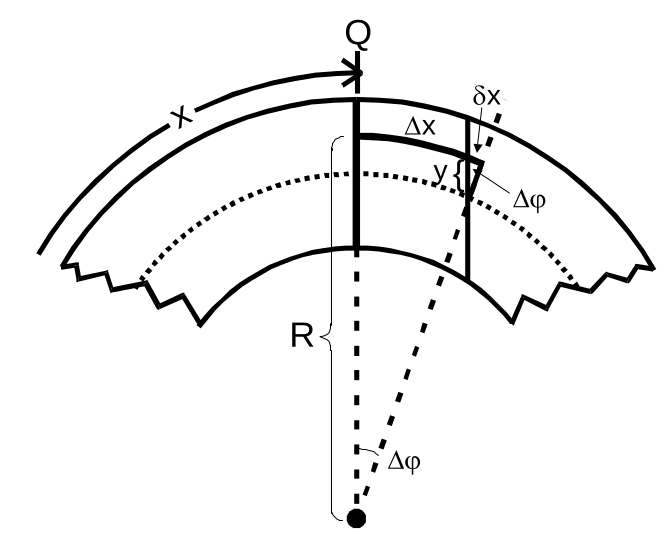
\includegraphics[scale=0.4]{content/EinspannungEinseitig2.png}
  \caption{Schematische Abbildung des gebogenen Stabes zur Bestimmung der Normalspannung. \cite{AP01}}
  \label{fig:einspannungeinseitig2}
\end{figure}
\noindent
Unter Verwendung von Gleichung \eqref{eqn:normalspannung}, Gleichung \eqref{eqn:kleindeltax} sowie der Näherung
\begin{equation*}
  \frac{1}{R} \approx \frac{d^2 D}{d x^2}
\end{equation*}
ergibt sich für die Normalspannung
\begin{equation}
  \sigma (y) = E y \frac{d^2 D}{d x^2}.
  \label{eqn:normalspannung2}
\end{equation}
Setzt man nun in die Momentengleichung \eqref{eqn:momentengleichung2} den so erhaltenen Ausdruck \eqref{eqn:normalspannung2}
für die Normalspannung ein, erhält man
\begin{equation}
  E \frac{d^2 D}{d x^2} \int_Q y^2 dq = F(L - x).
  \label{eqn:momentengleichung3}
\end{equation}
Hierbei wird der in \eqref{eqn:momentengleichung3} auftretende Term
\begin{equation}
  I := \int_Q y^2 dq(y)
  \label{eqn:trägefläche}
\end{equation}
als Flächenträgheitsmoment bezeichnet.
Aus Gleichung \eqref{eqn:momentengleichung3} kann nun durch Integration die Durchbiegung $D(x)$ bestimmt
werden:
\begin{equation}
  D(x) = \frac{F}{2 E I} \left( L x^2 - \frac{x^3}{3} \right).
  \label{eqn:durchbiegungeinseitig}
\end{equation}
Hierbei gilt $0 \leq x \leq L$.
Das Flächenträgheitsmoment \eqref{eqn:trägefläche} ergibt sich speziell für einen eckigen Stab zu
\begin{equation}
  I = \frac{1}{12} a^3 b
  \label{eqn:I1}
\end{equation}
wobei $a$ und $b$ die Kantenlängen des Stabes bezeichnen. Für einen runden Stab mit Radius $R$ ergibt sich
das Integral \eqref{eqn:trägefläche} zu
\begin{equation}
    I = \frac{\pi}{4} R^4.
    \label{eqn:I2}
\end{equation}
\subsection{Berechnung der Durchbiegung bei beidseitiger Aufhängung}
\label{sec:beidseitigg}
Im folgenden Abschnitt wird nun die Durchbiegung eines homogenen Stabes bei beidseitiger Aufhängung untersucht.
Hierfür wird der in Abbildung \ref{fig:beidseitig1} schematisch dargestellte Aufbau verwendet.
\begin{figure}[H]
  \centering
  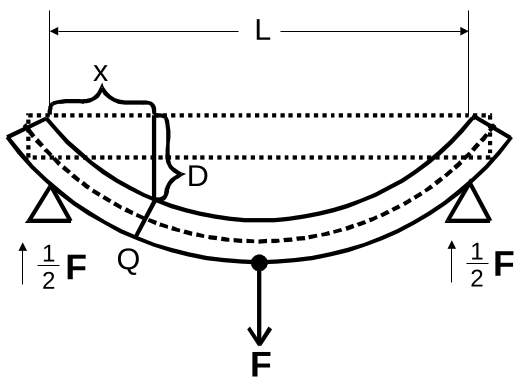
\includegraphics[scale=0.4]{content/Beidseitig.png}
  \caption{Durchbiegung eines elastischen Stabes bei beidseitiger Aufhängung. \cite{AP01}}
  \label{fig:beidseitig1}
\end{figure}
\noindent
Hier ergibt sich durch die Kraft $F$, ganz analog zu \ref{sec:einseitigg}, ein Drehmoment.
Durch die beidseitige Aufhängung hat dies nun für $0 \leq x \leq L/2$ die Form
\begin{equation}
  M_F = - \frac{F}{2}x
  \label{eqn:drehmomentbeidseitig1}
\end{equation}
und für $L/2 \leq x \leq L$ die Form
\begin{equation}
  M_F = -\frac{F}{2} (L - x).
  \label{eqn:drehmomentbeidseitig2}
\end{equation}
Unter Verwendung dieses Drehmoments ergibt sich eine Momentengleichung:
\begin{equation}
  \frac{d^2 D}{d x^2} =  - \frac{F}{E I} \frac{x}{2}
  \label{eqn:momentengleichungbeidseitig1}
\end{equation}
für $0 \leq x \leq L$ sowie
\begin{equation}
  \frac{d^2 D}{d x^2} = - \frac{1}{2} \frac{F}{E I} (L - x)
  \label{eqn:momentengleichungbeidseitig2}
\end{equation}
für $L/2 \leq x \leq L$.
Integriert man Gleichung \eqref{eqn:momentengleichungbeidseitig1} und Gleichung \eqref{eqn:momentengleichungbeidseitig2},
erhält man unter Verwendung der Tangentialbedingung
\begin{equation}
  D(x) = \frac{F}{48 E I} \left( 3 L^2 x -4 x^3 \right)
  \label{eqn:durchbiegungbeidseitig1}
\end{equation}
für $0 \leq x \leq L$ und
\begin{equation}
  D(x) = \frac{F}{48 E I} \left( 4 x^3 -12 L x^2 +9 L^2 x-L^3 \right)
  \label{eqn:durchbiegungbeidseitig2}
\end{equation}
für $L/2 \leq x \leq L$.
\\
Aus den Gleichungen \eqref{eqn:durchbiegungeinseitig}, \eqref{eqn:durchbiegungbeidseitig1} sowie \eqref{eqn:durchbiegungbeidseitig2}
lässt sich nun durch Umformen das Elastizitätsmodul bestimmen.
